
\newrefsection

%\textbf{B1.a. Extended Synopsis of the scientific proposal}

\chapter{B1.a. Extended Synopsis of the scientific proposal}\label{part1}

\eu{(max 5 pages)}

\eu{The Extended Synopsis should give a concise presentation of the scientific
proposal, with particular attention to the ground-breaking nature of the
research project and the feasibility of the outlined scientific approach.
Describe the proposed work in the context of the state of the art of the field.
References to literature should also be included. References do not count
towards the page limits. It is important that this extended synopsis contains
all essential information including the feasibility of the scientific proposal
since the panel will only evaluate Part B1 at step 1.}

%\section{Long-term vision and ground-breaking nature of the project}

\section{Project overview and beyond-state-of-art objectives}

Building socially intelligent agents is the next frontier for artificial
intelligence. Be it avatars in virtual worlds or social robots interacting with humans,
these artificial social agents always need to represent and reason about their
social environment. As humans, we have built through experience an intuitive
understanding of our social world; for an artificial intelligence, however, this
is a fundamentally open problem: as of today, we do not know how to automatically
model real-world social situations, and even less so in an automatic yet generic way.

\begin{wrapfigure}[11]{l}{0.6\linewidth}
    \centering
    \vspace{-10pt}
    \includegraphics[width=\linewidth]{interaction.jpg}
    \label{fig:interaction}
    %\caption{Test}
\end{wrapfigure}

\noindent I framed this problem in~\cite{webb2021framing}, and the picture on
the left provides one example: three people are engaged in the same conversation
but display different expressions and moods.  As humans, and even without
additional context, we can already infer much: for instance, we understand that
one person is leading what appears to be a lively conversation.  Other persons
are certainly present, yet out of the frame. The expression on the person in the
middle shows a amused frown, suggesting that, while enjoying the interaction,
she may interject soon. The person on the left seems to be passive or worried,
and maybe less engaged.  Overall the interaction presents as a positive one,
probably a group of friends spending some social time together, and if an
artificial agent were present in the scene, it should act accordingly.
\textbf{Yet no AI system is today able to make these inferences, and represent
the overall situation in a way that would be practical for an AI system to
reason about and make decisions}.

\begin{framed}

\bf\noindent \project will research and deliver the first computational model
able to transform arbitrary social situations into compact,
semantic-preserving mathematical representations. These representations will
be directly usable by machine-learning based AI systems, and will enable a
new generation of socially-aware artificial agents.

\end{framed}

Existing approaches either focus the modelling of large scale social structures
(using e.g. social graphs or probabilistic agentic
models~\cite{nunes2014social}), or task-specific models. The former, while
useful for e.g. macroscopic social simulations, are of little use for an agent
embedded in a particular situation (where it needs to build in real-time a model
of a unique, dynamic, only partially observable social situation). The later are
fragmented, and proposed methods are either too abstract for
implementation~\cite{gordon2016commonsense}, or too narrow in their scope to
provide a complete picture of the social environment (examples include for
instance group activity recognition~\cite{shu2017cern,wu2019learning},
pedestrians modelling for robotic social navigation~\cite{alahi2016social},
on-going state of an interaction~\cite{garcía2020explainable}). We are lacking a
more principled, general computational model to represent and reason about
complex social situations. As put by Scassellati in the \emph{Science Robotics}'
list of ten Grand Challenges for Robotics~\cite{yang2018grand}: \emph{we have
very few comprehensive, quantitative analyses of human social responses}.
\project aims at a breakthrough on that question by introducing the
fundamentally new idea of \emph{social embeddings}.


\subsection{Core concept of \project}

Inspired by how Large Language Models (LLMs) are able to encode complex social
semantics, \project exploits these models to introduce a computational model
based on \emph{social embeddings}.

\emph{Embeddings} are a (learned)
mathematical representation of a typically high dimension input into a
lower-dimensional space. Critically, however, embeddings
are trained to encode the relationships and semantic nuances that might exist in
the original input space.
%For instance, two pictures of the same face
%transformed with an embedding tuned for facial recognition would yield two
%vectors that are similar to each other, i.e., close to each other for a given
%metric like the cosine distance.
As such, the embedding process not
only condenses high-dimensional information into a more manageable form but also
captures latent associations that might otherwise remain
obscured~\cite{bengio2009learning}.
Work on embeddings has recently yielded spectacular results in language
processing, with the advent of so-called Large Language
Models~\cite{devlin2019bert,wolf2020transformers}. These models rely themselves
on text-level embeddings, representing input texts as a numerical
vectors~\cite{reimers2019sentencebert,muennighoff2022sgpt} that effectively
encode, for instance, the semantic relatedness between the original texts~\cite{thakur2021beir}.

Combining social situations and text embeddings, \project aims at creating and
characterising \emph{social embeddings}, i.e. a compact numerical
representation of a social situation, as experienced by an agent
immersed in that social environment. 
%At their basic level, \emph{social
%embeddings} consist in text descriptions of social situations, viewed from the
%agent's perspective, that are then
%projected in the embedding space by a text embedder.
The key insight is that of exploiting the social knowledge already encoded in
the latent space of state-of-art large language models. I do so by
generating a complete textual description of the social environment of the agent
(using for example the existing perception capabilities of a social robot), and
by transforming this description into a text embedding via a large language
model.  It follows from that construction that, similarly to general text
embeddings, social embeddings encode the \emph{semantics} of the social
situation currently experienced by the agent, facilitating the interpretation of
the situation: comparing two social situations, for instnace, becomes as
simple as computing a distance between their respective embedding vectors
(Figure~\ref{fig:social-embeddings}). We effectively construct a \emph{social
embedding}, i.e., \emph{a semantics-preserving projection of the social space
into a machine-friendly numerical space}.


\begin{figure}[H]
    \centering
    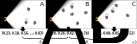
\includegraphics[width=0.9\linewidth]{figs/social-embeddings}
    \caption{In this example (and assuming the perspective of the yellow
    robot), scenes A and B  are more related to each others (one person
    walking towards the robot, with an independent group of people chatting
    in the background), than with C, where the robot is already engaged in
    an interaction.  Social embeddings make it possible to e.g. compare such
    social situations using a simple distance between vectors.}

    \label{fig:social-embeddings}
\end{figure}


Formally, if we denote $\mathcal{S}$ the set of social situations, the
\emph{social embedding} process has three steps: (1) a \emph{descriptor
extraction} step $D : \mathcal{S} \to \{\mathcal{D}\}$, with $\mathcal{D}$ the
set of descriptors that can be used to characterise a given social situation
(for instance, relative distances between people, facial expressions, group
membership), its physical environment (e.g. objects, location) and its context
(e.g. current task); (2) a \emph{description} step $T: \{\mathcal{D}\}^k \to
\mathcal{P}$, with $\mathcal{P}$ the set of textual descriptions, that combines
descriptors over $k$ previous timesteps into a coherent text-based description
of the on-going social situation, also implementing pruning strategies to avoid
the combinatorial explosion of possible descriptors combinations; and (3) the
embedding process itself $E : \mathcal{P} \to [0;1]^n$, mapping the textual
description to its embedding, i.e.  a vector of dimension $n$. $E$ is
performed using as a deep neural network, pre-trained on large datasets of natural
language.

Repeated anecdotal evidence shows that the current generation of off-the-shelf
LLMs (for instance, OpenAI's GPT-4) already has strong abilities to reason about
social scenes, including when directly using relatively low-level social signals
like facial action units~\cite{paul2005what}, to infer the high-level state of
a social situation (for instance, whether the interaction between two persons is
going well). As such, I do not plan in \project to train from scratch a large
language model, and accordingly, the project's focus is not on the acquisition
of large datasets of social interaction. Instead, I will perform model
fine-tuning on social tasks, using several existing datasets of interactions, as
detailed hereafter.

%
%The basic idea of \emph{social robots} refers to robots that are situated in a
%human social environment. In this context, we expect social robots to exhibit
%\emph{social situation awareness}, i.e. to appraise and maintain a model of the social
%situation in which they are embedded. Depending on the role of the robot, this
%might include understanding who is present, who is interacting with whom, which
%are the resulting groups,  what are the in-group roles,  etc.
%
%social situation awareness, as a socio-cognitive skill, is essential for the robot to e.g.
%act in a context-sensitive manner; reason and apply social norms (for instance,
%do not navigate in the middle of a group, or do not suddenly interrupt a
%conversation); or create proactive social agents (in order to acknowledge and
%respond to a human who would like to engage with the robot, the robot must first
%adequately model and recognise the corresponding social situation).

%This can only be achieved if robots are endowed with the ability to represent
%not only their physical environment, but also their social environment and
%context. The \project project aims at designing, implementing and characterising
%a radically novel method to achieve this goal, based on the concept of
%\emph{embedding}: a low-dimensional, semantics-preserving, mathematical
%representation of a high-dimensional input (Figure~\ref{fig:social-embeddings}).
%Starting from a proof-of-concept of \emph{social embeddings} that I recently
%published~\cite{lemaignan2024social}, \project develops and fully characterise
%the concept of \emph{social embeddings}, that applies, for the first time, the
%idea of building a compact numerical representation to the complexity of social
%interactions and social dynamics.


%
%At a scientific level, 
%\TODO{articulate scientific impact}
%
%Finally, \project is also about asserting and reinforcing the European
%leadership in AI and intelligent robotics, in line with EU strong societal
%values: a physical AI system able to represent and reason about its social
%environment is also a system that can be designed to have an acceptable and
%positive social impact, in line with the European objectives for socially
%responsible AI. \project can directly contribute to these goals: the science and
%technology that underpins the project \textbf{provide an important contribution
%in securing a safe and responsible digital future in Europe}, as well as
%\textbf{\project building the capacity in Europe to develop socially intelligent
%embodied AI systems}. 

\subsection{Research objectives}

%\project is built around three axes: a basic research programme; an experimental
%programme that looks specifically at the application of social embeddings to
%social robotics; and, running in parallel to those first two axes, a scientific
%investigation of the ethical dimension of social embeddings.

This idea of \emph{social embeddings} builds on a proof-of-concept that I
validated in~\cite{lemaignan2024social}. \project will turn that early concept
into a mature computational model for artificial social agents: I will formalize
their construction,  fully characterise their properties, expand their scope to
complex, real-world social situations, and demonstrate their transformative
potential through an ambitious experimental programme that includes the application of
the model to AI-driven characters in an online multi-player game, and
its deployment on a social robot in an hospital environment.

As such, \project has the following objectives:

\begin{enumerate}[label=\textbf{O\arabic*}]
    \item \label{O1} To \textbf{construct and characterize the fundamental
        properties of social embeddings}: build compact, yet
        semantics-preserving, embeddings to represent arbitrary social
        situations; and fully characterize these embeddings, including their
        latent semantics.

    \item \label{O2} to precisely \textbf{define and implement the socio-cognitive skill of
        \emph{social situation awareness}, enabled by social embeddings}. This
        includes context-aware \emph{social appraisal};
        \emph{social prediction}, by extrapolating the trajectories of on-going social situations in the
        embedding space; and \emph{social learning}, by augmenting existing interactive machine
        learning (IML) techniques with representations of the social situation;

    \item \label{O3} To fully {\bf integrate the \project computational model onto a
        socio-cognitive architecture for socially intelligent artificial
        agents}, augmenting existing cognitive architectures with social
        awareness, while ensuring real-time properties;

    \item \label{O4} To conduct an {\bf ambitious experimental programme} that
        includes social observations, lab-based studies, as well as
        application-focused real-world demonstrators -- including both AI agents in a
        virtual, multi-player world, and deployment on a social robot, in
        collaboration with the Paris-based Broca hospital -- to evidence the
        effectiveness of social embeddings in complex, real world conditions.

\end{enumerate}


%Once completed, these four objectives will provide solid theoretical and
%empirical foundations to social embeddings.
%
%Each of these four objectives involve both basic and experimental research,
%presented in the next section.


%%%%%%%%%%%%%%%%%%%%%%%%%%%%%%%%%%%%%%%%%%%%%%%%%%%%%%%%%%%%%%%%%%%%%%%%%%%%%%%

\section{Methodology and implementation}
%\section{Feasibility of the project}

\project delivers on its programme by combining a range of scientific methods,
embedding-based data representation being the central computational paradigm
underpinning the project.  I briefly outline hereafter the four main work
packages, with the key research methods that I will employ in each of them.

%From a computational point of view, it relies
%on specialized deep learning models to generate the source descriptors, and
%knowledge graph and propositional logic to combine descriptors into full text
%descriptions. The selection of descriptors and their combination is however also
%informed by social psychology and sociology, and I accordinlgy perform
%qualitative field observations of social situations.

%\TODO{make sure we have tasks for that}

%The analysis of the resulting embeddings uses... \TODO{complete}

%machine learning large language models fine-tuning and embedding learning learning;
%user-centered design; ethnographic and sociological investigation; expressive
%non-verbal communication; embodied cognition; symbolic AI; neural nets and
%sub-symbolic AI; interactive machine learning.


%The first one, \emph{\WPA}, focuses on basic research; the second
%one, \emph{\WPB}, focuses on the artificial socio-cognitive skills enabled by
%social embeddings; the third one, \emph{\WPC}, specifically look at the
%application and impact on social robots; and the final one, \emph{\WPD},
%organises the experimental work.


\subsection{WP1: \textbf{\WPA} 
           {\newline\footnotesize\normalfont [Y1--Y3.5; one post-doc in
data-driven sociology; one post-doc + one PhD student in deep learning]}}

WP1 addresses Objective \textbf{O1}. Social embeddings construction requires
first to extract descriptors, then to build complete textual descriptions, and
finally to embed these descriptions. I will first systematically investigate
these three steps, and then characterize the resulting embeddings.

I will extract basic social descriptors using the ROS4HRI social perception
framework~\cite{mohamed2021ros4hri}, as it formalize a multi-modal model of
humans~\cite{lemaignan2022ros}, and run in real-time on current systems. I will
augment these basic descriptors with more complex percepts, including (1)
descriptors of human-objects interactions (HOI), using transformer-based
techniques like~\cite{iftekhar2022what} ; (2) affective
descriptors~\cite{vinciarelli2009social}, using e.g. facial expressions based on
facial action units classification~\cite{martinez2019automatic}; (3) group-level
interactions, including $f$-formations~\cite{setti2015fformation}, and group
activity recognition, using deep convolutional graph techniques like
ARG~\cite{wu2019learning}.

%(3) a novel contextual model of
%attention~\cite{ferrini2024percepts} that allows fine-grained assessment of what
%the person around the robot are focusing on.

The generation of textual descriptions consists in both the combination of
descriptors into textual \emph{snapshots} of the social environment at a
specific time, and the combination of these snapshots over time, to build a
textual description of complete \emph{situations} with a time horizon of 10s to
25s~\cite{netanyahu2021phase}. I will initially build snapshots using text
templates, and then extend the methodology using techniques based on
social knowledge graphs~\cite{sap2019atomic} and propositional
logic~\cite{tsoi2022sean}. The combination of snapshots into social situations
will be developed with the help of the PHASE social simulator and
dataset~\cite{netanyahu2021phase}, that includes a large number of annotated
social interaction sequences.

Last, the text embedding process itself. Due to the fast pace of progress in the
LLMs landscape, it is likely that current
methods (including e.g.~\cite{reimers2019sentencebert,muennighoff2022sgpt}) will
have been superseeded by new methods. I will closely monitor
advances in the domain, especially on the question of semantic
relatedness~\cite{thakur2021beir}, as this is critical for social
embeddings. I plan to perform fine-tuning~\cite{hadsell2006dimensionality}
of the selected text embedders to specialize them for social situation
representation. I will do so by leveraging existing open-access annotated
datasets of social interaction like AMI~\cite{carletta2007ami},
D64~\cite{oertel2013d64}, INRIA's SALSA~\cite{alameda2015salsa}, or my own SoGrIn
dataset~\cite{webb2023sogrin}, and datasets of social questions-answers like
SocialIQa~\cite{sap2019social}.

I will then characterise social embeddings, starting with the basic properties
that I identified in~\cite{lemaignan2024social} (invariance to syntax, social
similarity and continuity) and focusing next on the broader characterization of the
topology of the embedding space, using pairwise distance computation techniques
recently proposed by~\cite{sun2023topological}.

%\vspace{1em}
%\noindent\emph{ Timeframe: Y1--Y3.5; one post-doc (PD1) with expertise in
%data-driven sociology; one post-doc (PD2) in deep learning/text embedding; one
%PhD student (PHD2) in deep learning.}


\subsection{WP2: \textbf{\WPB} 
           {\newline\footnotesize\normalfont [Y1--Y4; one post-doc in cognitive science + one PhD student in data-driven sociology]}}

Work package WP2 focuses on research objectives \ref{O2}: to frame and build a
`social situation awareness' cognitive skill for artificial social agents, 
by interpreting the \project computational model in terms of (1) context-aware
social situation appraisal, (2) social prediction, and (3) application to social
learning.

%\emph{social situation awareness} is a socio-cognitive skill that is essential for
%artificial social system, like social robots, to e.g.  act in a
%context-sensitive manner, reason and apply social norms,
%or create proactive social agents (in order to acknowledge and respond to a
%human who would like to engage with the robot, the robot must first adequately
%model and recognise the corresponding social situation).


% METHODS for the 3 objectives?
%- appraise social situations, also taking into account the social context
%- learn socially-appropriate behaviours
%- anticipate future social states


\emph{Social appraisal} is about interpreting the results of WP1
in terms of social situations. This includes, in particular, mapping regions of
the embedding space to known social situations.
% latent semantics: for instance, the three social descriptions `two
% persons people walking together while chatting', `two persons arguing together'
% and `two persons walking towards me, looking agitated', while sharing syntactic
% similarities, represent distinct social situations, and, consequently, their
% embeddings would belong to distinct regions in the embedding space. Identifying
% and labelling protoypical clusters to characterize the semantic topology of the
% embedding space will be achieved by exploiting
% existing annotated datasets to identify and extract prototypical reference
% social situations.
To do so, I will first create a taxonomy, represented as a knowledge graph, of
social situations. This taxonomy will be grounded in literature
(e.g.~\cite{kelley2003atlas}) and in my own field observations (WP4).  Using
knowledge graph embedding techniques~\cite{ji2022survey}, I will research
possible isomorphisms between social embeddings and the embedding of this
expert-build social situation taxonomy. As a result, it should be possible to
automatically characterize any new observed social situation in term of its
relatedness to prototypical situations, referenced in the taxonomy.

Context representation is integral to social situation appraisal: depending on
the context, the interpretation of a social situation might vary wildly,
something that current approaches struggle to represent~\cite{yang2018grand}. I
will verify the hypothesis that large language models implicitly encode social
context as well: for instance, the embedding of a description like `\emph{I am
telling a joke and people are laughing}' (congruent context: people are expected
to laugh) should be consistently closer to the embedding of `\emph{The social
situation is going well}' than a description like `\emph{I am taking orders from
the patrons and they are laughing}' (incongruent context: people are not expect
to laugh in this context).

Next, I will analyse how \emph{social dynamics} are represented in the \project
model. Since each social situations is represented as a \emph{point} in the
social embedding space, \emph{sequences} of situations then become
\emph{trajectories}. This opens a radically new venue to represent and reason
about social dynamics. For instance, \emph{velocity} in the embedding space
would reflect the rate of social change in the social space; trajectory
\emph{extrapolation} would allow in principle social situation prediction;
\emph{discontinuities} in the embedding space would reflect brutal social
changes that could trigger specific behaviours by the artificial agent
(acknowledgement, attempt to repair).  I will further research the potential
mappings between embedding-space trajectories, and real-world social space, to
structure this new research space.

Finally, I will look into how social embeddings can facilitate interactive
machine learning (IML) of socially-appropriate behaviour policies. This task is
an extension of the work I conducted with my students on IML, showing promising
results for learning long-term social policies in real-world
applications~\cite{senft2019teaching, winkle2020couch} that fully involve the
end-users through continuous learning~\cite{winkle2018social}. This previous
work also identified the lack of social context representation as a key
obstacle to learn contextualised social policies: the \project model should
directly address this question.

%\vspace{1em}
%\noindent\emph{Timeframe: Y1-Y4; one post-doc PD3 in cognitive sciences; one PhD student in data-driven sociology (PHD1)}

\subsection{WP3: \textbf{\WPC} 
           {\footnotesize\normalfont [Y2--Y4; one PhD student in cognitive robotics]}}

This work package corresponds to Objective~\ref{O3} and focus on the integration
of the \project computational model in a practical cognitive architecture for
autonomous social agents. It will effectively enable the experimental programme
of \project in WP4.

This work will build on my extensive experience in designing and implementing
cognitive architectures for social robots~\cite{lemaignan2017artificial,
lemaignan2015pyrobots,lemaignan2011what}.  Indeed, while the work package will
also cover disembodied virtual agents, the main focus is on integrating social
awareness into a cognitive architecture for embodied agents. I will develop the
required perceptual and behavioural capabilities of the robot, implement the
real-time generation of social embeddings, and integrate together a principled
socially-aware agent supervisor, that exploits social embeddings.

As \project focuses specifically on the AI engine of the robot, I will use an
existing off-the-shelf social robot, a PAL Robotics TIAGo Pro, that offers
out-of-the-box advanced human perception based on the ROS4HRI
framework~\cite{lemaignan2022ros}. It also offers on-board GPU options that are
appropriate to implement a fully AI-based autonomous system. I have extensive
experience with this platform, having actually directly taken part to its design
and software stack implementation while employed at PAL Robotics.

I will be using publicly available resources, including machine learning
backbones and state-of-art open-source pre-trained Large Language Models
(foundational models) like Llama2~\cite{touvron2023llama}; I have shown
in~\cite{lemaignan2024social} that simple social embeddings can already
be generated in near-real time on consumer-grade GPUs, and I do not anticipate
that \project will required unusual compute resources that would require
dedicated budget.

%\vspace{1em}
%\noindent\emph{Timeframe: Y2-Y5; one PhD student (PHD3) in cognitive robotics.}

\subsection{WP4: \textbf{\WPD} {\footnotesize\normalfont [Y1.5--Y5; whole research team]}}

Finally, WP4 organises the experimental work, and aim at achieving~\ref{O4}. I
intent to run (1) qualitative field observations, supervised by one researcher
in data-driven sociology (PD2), to e.g. ground our taxonomy of social situation
(WP2); (2) controlled experiments in lab settings to evidence the basic
properties of social embeddings, their translation in terms of social situation
awareness, and social dynamics representations, as well as (3) more complex
deployments in real-world, naturalistic settings, to demonstrate how the
\project model might push the boundaries of artificial social intelligence for
virtual agents and service robots.

As an example of controlled experiment, I will adapt to social
robotics~\cite{lemaignan2015mutual} experimental protocols originally designed
by Frith and Happé~\cite{frith1994autism} to investigate social representation
and mental modelling in autistic children. This protocol include tasks like
distinguishing \emph{happiness} or \emph{sadness} from \emph{surprise}, or
distinguishing \emph{sabotage} from \emph{deception}: these nuances, quite
self-explanatory to experienced social agents, require subtle modelling of the
context and mental state of agents, and, until now, have not been successfully
reproduced in artificial agents. I aim to show that social embeddings offer a
generic methodology to implement this kind of advanced social understanding.  I
present in Part B2 two additional studies covering other aspects of social
cognition.

I also plan two larger studies. The first one will be set in a Massively
Multiplayer Online game (MMO), where I will program autonomous bots to play
alongside human players.  These agents will be controlled by the cognitive
architecture developed in WP3, with the social awareness component conditionally
enabled or disabled. I will review at the start of the work package whether I
use an existing MMO platform (like~\cite{schatten2017agents,tsoi2022sean}), or
extend one of the previous online multi-player games I created to study social
interactions~\cite{webb2022measuring,lemaignan2023officebots}

The second one will be conducted in collaboration with the Broca hospital, a
geriatic hospital with a strong track record of experimentation with robots and
dedicated facilities.  Building on my fieldwork experience
(e.g.~\cite{hood2015when,mondada2015ranger,winkle2018social,cooper2023challenges}),
and my on-going collaboration with Pr. Maribel Pino, coordinator of the Broca
Living Lab, I will deploy an autonomous social robot for several weeks, using
social embeddings to implement a level of social situation awareness and social
appropriateness not yet achieved in this type of application.

%\vspace{1em}
%\noindent\emph{Timeframe: Y1-Y5; with involvement of the whole research team}

%
%My extensive track-record of fieldwork and real-world robot deployments (in a
%broad range of environments, including schools~\cite{hood2015when,
%lemaignan2016learning, jacq2016building,
%baxter2015wider,kennedy2016cautious,senft2018robots,lemaignan2022social}, at
%people's home~\cite{mondada2015ranger}, in public
%spaces~\cite{alhafnawi2022deliberative}, or in healthcare
%environments~\cite{winkle2020couch,cooper2023challenges}).
%
%
%\TODO{need to be SMART: reference specific techniques + metrics}

%
%\subsection{Additional workpackages}
%
%Because the development of socially-intelligent robots has
%complex ethical ramifications -- including the potential of alienating
%human users, \project also includes an explicit research component on
%Responsible Robotics. In particular, the project will aim to contribute directly
%to the on-going roadmap for Responsible Robotics, specifically
%investigating the interplay between social embeddings, transparency and human
%agency. The work will be conducted in workpackage WP4.

%
%Social embeddings, by enabling artificial systems to model and reason on their
%social environment, have the potential of significantly increase the social
%competencies of e.g. robots, also raising ethical questions.
%
%I am part of an international working group on Responsible Robotics~\TODO{cite
%Dagsthul roadmap arxiv}...
%
%WP6 aims at establishing the conceptual and ethical framework around the idea of
%\emph{robot-supported human-human interactions}. It does so by co-creating
%patterns of interaction and norms with the general public, using a unique
%combination of ethnographic observations and `crowd-sourced' interaction
%patterns.
%
%\vspace{1em}
%\noindent\emph{Timeframe: Y3-Y5; one senior post-doc (PD3)
%with background in ethics of technology and responsible innovation.}



%
%A final workpackage WP5 groups all the task related to the grant management, as
%well as the dissemination and exploitation tasks. Details of the dissemination
%and exploitation activities are provided in Part B2 of the proposal.


%%%%%%%%%%%%%%%%%%%%%%%%%%%%%%%%%%%%%%%%%%%%%%%%%%%%%%%%%%%%%%%%%%%%%%%%%%%%%%%%%%%%
%%%%%%%%%%%%%%%%%%%%%%%%%%%%%%%%%%%%%%%%%%%%%%%%%%%%%%%%%%%%%%%%%%%%%%%%%%%%%%%%%%%%
%%%%%%%%%%%%%%%%%%%%%%%%%%%%%%%%%%%%%%%%%%%%%%%%%%%%%%%%%%%%%%%%%%%%%%%%%%%%%%%%%%%%

\section{Research group}

I plan to conduct the \project project at the French Institut National de
Recherche en Informatique et Automatique (INRIA), a world-leading institution in
computer science and robotics. While I will create and manage my own team, I
will closely collaborate with the INRIA RobotLearn team (Dr. Xavier
Almeida-Pineda), whose unique expertise in machine learning applied to robotics
complement well my own expertise in social robotics.  I will dedicate 70\% of my
time to \project, keeping the other 30\% for team management, general
institutional and academic engagement and other collaborations beyond the
\project project. In addition, I plan to recruit six researchers: two
researchers with expertise in deep machine learning and large language models
(one senior post-doc, one PhD student); two researchers with expertise in
data-driven socio-psychology (one senior post-doc, one PhD student); one
researcher in cognitive sciences (post-doc); and finally one researcher in
cognitive robotics (PhD student).

%%%%%%%%%%%%%%%%%%%%%%%%%%%%%%%%%%%%%%%%%%%%%%%%%%%%%%%%%%%%%%%%%%%%%%%%%%%%%%%%%%%%
%%%%%%%%%%%%%%%%%%%%%%%%%%%%%%%%%%%%%%%%%%%%%%%%%%%%%%%%%%%%%%%%%%%%%%%%%%%%%%%%%%%%
%%%%%%%%%%%%%%%%%%%%%%%%%%%%%%%%%%%%%%%%%%%%%%%%%%%%%%%%%%%%%%%%%%%%%%%%%%%%%%%%%%%%

\section{Feasibility and impact of the \project project}

The main foreseen risk to the \project project is the failure to establish a
stable mapping between real-world social situations and the social embedding
space (Objective~\ref{O2}). I have already partially mitigated this risk by
running a series of prototypes~\cite{lemaignan2024social} showing promising
early results, and the \project research team is designed to bring in the
required additional know-how. I might however benefit from access to additional
domain expertise in neural network latent space analysis, which I will secure
through the \project Scientific Advisory Board (presented in Part B2), whose members will include leading figures in the field.

Other major risks include (1) the lack of sufficiently large datasets of
annotated social interactions to fully characterize social embeddings. This is a
medium risk, as the project is designed so that existing public datasets would
be sufficient. It might however be further mitigated by reducing the breadth of
social situations that I consider; (2) difficulties to deploy an autonomous
social robots in a real-world environment. Since this is one of my core
expertise, this is only a medium risk, that can be further mitigated by reducing
the effective level of autonomy of the robot during the experiments.

If those risks are successfully managed, \project will have a major scientific
impact by realising a breakthrough on the \emph{wicked
problem}~\cite{west1967wicked} of representing and automatically reasoning about
our social environment.  By introducing the fundamentally new idea of
\emph{social embeddings} as a data-driven and semantics-preserving computational
representation of contextualized social situations, the \project computational
model represents a paradigm shift for the domain: it paves the way to generic,
task-agnostic representations and quantitative measurement of the social
situations in which social agents are embedded, something that was until now
only possible using time-consuming qualitative methodologies or
non-generalizable model-based techniques.

\begin{framed}
As such, \bf the output of \project has the potential to significantly
accelerate the development of generic artificial agents that are socially-aware,
also creating an interdisciplinary bridge between the current trends in AI, machine
learning, virtual worlds, social robotics, and the broad family of discipline relying on
data-driven social sciences.
\end{framed}


\newpage

\printbibliography



%\vspace{0.5em}
%\begin{itemize}
%
%    \item What are the conceptual, algorithmic and technical prerequisites to
%        design and implement such an autonomous \& responsible robots? in
%        particular, what social context understanding and (machine) learning
%        architectures are required to \textbf{enable long-term autonomy} and,
%        eventually, \textbf{engagement} between a robot and its end-users?
%
%    \item What are the conditions and methodologies enabling large scale data
%        acquisition of \textbf{real world, user-driven robots behaviours}? How
%        to then train robots to become \textbf{progressively autonomous}?  And
%        ultimately, how to balance \textbf{autonomy} of the robot with the
%        necessary \textbf{behaviour transparency} and \textbf{human oversight}?
%
%    \item What are the public expectations with respect to the role of social
%        robots, and how can we \textbf{collaboratively design}
%        \textbf{autonomous}, yet \textbf{responsible, beneficial, socially
%        acceptable robots}?
%
%\end{itemize}
%
%\vspace{0.5em}
%\noindent From these questions, I derive the following four objectives that are
%the guiding principles of my research programme, both in the short term, and at a
%10-15 years horizon:


%\subsection{Work plan outlook}
%
%My research programme could begin rapidly, using publicly available resources,
%including machine learning architectures like Transformers, combined with open-source
%pre-trained Large Language Model backbones; and state-of-art HRI tools like
%ROS4HRI~\autocite{mohamed2021ros4hri} to represent in real-time the social
%environment of the robot. While long and complex data collection campaigns would
%have to be organised, and training infrastructure would need to
%be designed, I expect initial results in the first 3 to 5 years.
%
%This is also a long-term vision: on the one hand, the rapid pace of progress
%of technology (novel deep machine learning architectures, novel HRI tools for
%human and scene understanding) continuously opens novel investigation
%venues; one the other hand, the success of my research vision hinges on
%real-world, long-term experimental work: deploying robots in the healthcare
%sector, creating the conditions for adoption by the end-users, running
%long-term deployments with the end-users are long terms aims
%,... these research activities will take
%place over long period of time.

%\subsection{Importance and impact}
%
%My research programme has the potential to be groundbreaking: until now,
%autonomous social robots have had little real world success. Experiments and
%deployments have been mostly limited to constrained application domains, where
%rigid action policies (scripts, task planners) could be sufficient. State-of-art
%robots however fail to handle the complexity and unpredictability of real world
%environments (like the ones encountered in the healthcare domain). In addition,
%these systems see poor field adoption due to several factors including
%difficulty of use, wrong expectations, perceived complexity.
%
%This research programme is also important: as socially assistive robots quickly
%develop, it is critical to equip ourselves with a deeper understanding and
%intellectual framing of what social robots \emph{could} and \emph{should} be,
%paving the way for their much broader adoption in the coming years: I will
%actively contribute to this aim, by leading the design and implementation of
%socially-intelligent robots that are socially useful, acceptable in the
%long-term, and ethically responsible, but also by furthering my engagement to
%interdisciplinary work, and broad engagement with the society and policy makers.







%%%%%%%%%%%%%%%%%%%%%%%%%%%%%%%%%%%%%%%%%%%%%%%%%%%%%%%%%%%%%%%%%%%%%%%%%




%How this general
%principle translates into specific guidelines and algorithms -- while taking into
%account the principles of a responsible AI -- is the central
%contribution of Work Package 1.

% This socially-driven goal forms what we call a \emph{social
%teleology}. its own goals have this objective can only be achieved if the
%robot is \textbf{socially-driven}: the robot's behaviours must be driven by the
%intention to support positive human-human interactions. 


%I frame these hypotheses with the idea of \textbf{robot-supported human-human
%interactions}, a novel conceptual framework to `think' the future human-robot
%interactions. I will co-construct this framework through large scale public
%engagement: for a whole year, I will deploy the \project robot within the City
%Lab of Bristol's science centre \emph{WeTheCurious}, relinquishing the control
%of the robot to the visitors themselves. Tasked with remotely operating the
%robot to assist fellow visitors, I will accompany them in `inventing by doing' a
%new grammar of social interactions: what does it mean for a robot to help? How
%to do so in the dynamic, messy, environment of a science centre? What are acceptable
%behaviours? Can we see new social norms emerge? At the end of this experiment,
%we expect 1000s of people to have had experienced -- and co-designed -- how
%robots should interact with humans in a positive, helpful way, and each of these
%experiences will contribute to uncovering and designing the basic principles of
%social interaction for robots. This work is the focus of WP1.
%
%While most of the interactions in the science centre will be short-lived, two further
%large scale experiments will take place over the course of the project: a
%one-year experiment in one of Bristol's Special Education Needs (SEN) school,
%helping 250+ children with psycho-social impairments to develop their social
%skills; a second one-year experiment at the Bristol's children hospital, where
%the robot will join one of the wards where 30+ children with long-term conditions
%stay for months, and engage with the children into playful social activities: telling
%stories, triggering group activities with other children, providing additional
%social presence. In both these experiments, the robot behaviours will be
%co-designed with, and learnt from the end-users themselves: nurses, teachers,
%parents, and where possible, the children themselves.
%
%
%\section{Overview of the \project work programme}
%
%Socially intelligent robots require unique, beyond state-of-the-art,
%capabilities to \emph{(1)} understand the social interactions (social
%situation awareness), \emph{(2)} autonomously decide the best course of action for
%short-term and longer-term social influence, and \emph{(3)} perform the
%appropriate social actions and exert said influence in an appropriate,
%responsible manner.
%
%Not only the required technology is itself beyond state-of-the-art (and will be
%researched and integrated in WP2, WP3 and WP4), but the
%interplay between technology, socio-cognitive psychology, privacy and ethics is
%only starting to be researched and understood. \project offers an
%strong vision and an ambitious, evidenced-based, methodology to significantly
%advance our understanding of this multi-faceted problem.
%
%
%\begin{itemize}
%    \item \textbf{O1: conceptual framing} To construct a solid conceptual
%        framing around the multidisciplinary question of responsible human-robot
%        interactions, answering questions like: What should motivate the robot
%        to step in and attempt to help? or: What social norms are applicable to
%        the robot behaviours? Building on the extensive body of work on
%        Responsible AI, I will investigate the basic principles of
%        responsible robot-mediated social interactions, that must form the
%        foundations of a socially useful robot, accepted and used in the long
%        run.  Using user-centred design and participatory design methodologies,
%        I will identify the determinants and parameters of a responsible social
%        intervention, performed by a socially-driven robot, and formalise them
%        in practical principles.
%
%    \item \textbf{O2: physical-social representation and reasoning} To
%        effectively and responsibly interact with its environment, the robot
%        must first build a comprehensive and continuously updated model, from its
%        spatial and physical configuration, to its social dynamics. I will
%        design and develop a novel cognitive capability of artificial
%        \emph{social situation assessment} to enable the robot to represent
%        real-time social dynamics in its environment. I will achieve this
%        breakthrough by combining existing model-based approaches \TODO{refs}
%        (including my recent research on social state modeling \TODO{refs}, with
%        the expressive power of the new \emph{social embeddings} that I have
%        recently introduced.
%
%    \item {\bf O3: goal-driven, responsible decision making} I aim to create
%        robot behaviours that are perceived as purposeful and intentional
%        (long-term goals), while being shaped by a user-created and
%        user-controlled action policy.  I will integrate long-term social goals,
%        arising from the interaction principles of \textbf{O1}, with the social
%        modeling capability of \textbf{O2}, into a principled, goal-driven
%        cognitive architecture, with responsible AI guarantees. The breakthrough
%        will come from combining these long-term social goals with bottom-up
%        action policies, designed and learnt from the end-users using
%        human-in-the-loop attention-based machine learning.
%
%        I want to specifically test the following two hypotheses: first, that
%        long-term social goals, if suitably co-designed with the public and
%        stakeholders and properly integrated into the robot as a \emph{social
%        teleology}, will create the perception that the robot is intentional and
%        purposeful. This will in turn elicit sustained engagement from its human
%        users.
%
%        Second, that human-in-the-loop machine learning can be used to ensure an
%        additional layer of human oversight and a level of behavioural
%        transparency.  Human-in-the-loop reinforcement learning -- as
%        implemented in the SPARC approach that I have developed with my students
%        and already used in complex social
%        environments~\parencite{senft2017supervised,senft2019teaching,winkle2020insitu}
%        -- relies on an end-user `teacher'. This teacher initially fully
%        controls the robot (via teleoperation) while it learns the action
%        policy, and then progressively relinquishes control up to a point where
%        the robot is effectively autonomous. As I previsouly argued
%        in~\textcite{senft2019teaching}, this approach leads to increased
%        control and ownership of the system, and as a result, increased trust
%        from the end-users.
%
%
%    \item{\bf O4: ambitious field research} Finally, the last major objective of
%        my research project is to demonstrate the effectiveness of my approach
%        in complex, real-world conditions. This means deploying the socially
%        interactive robots in existing social \emph{ecosystems} that are
%        sufficiently complex and open to explore novel social interactions. My
%        objective is also to show that this real-world deployment can be
%        successfully driven by the `end-to-end' involvement of all the end-users
%        and stakeholders: from defining the robot's role, from the different
%        perspective of each end-user, to actually designing and `teaching' the
%        robot what to do.
%
%
%\end{itemize}


